\documentclass{article}
\usepackage[utf8]{inputenc}
\usepackage{graphicx} 
 
\begin{document}
    
\title{Topological analysis of classical and quantum telecommunication networks}
\author{Maria Gragera Garces}

\date{September 2022}

\maketitle

\begin{abstract}
    In this report we compare the resulting fidelity and time taken for end to end communications of different classical and quantum topological communications networks, with the intend of analyzing potential differences between classical and quantum networks on the sole base of topological set up.
    All test have been run in NetSquid, a discrete event quantum simulator designed for quantum networking.
\end{abstract}

    \section{Introduction}

    \paragraph{Quantum networks facilitate the transmission of quantum bits, also known as qubits, between quantum processors which can perform quantum logic gates.
    The nature of qubits and quantum logic gates is intrinsically different from their classical counterparts. Quantum logic gates are reversible, qubits adhere to a non binary encoding system, and respect quantum mechanic's rules, which modify their behaviour in certain settings when compared to bits.
    This hardware difference between both technologies has repercussions in the subsequent networks. As of today, quantum networks highly rely on the entanglement between qubits and node-to-node teleportation of information, which are not available in classical networks.
    When working with quantum networks, we can observe the effects of quantum mechanics in settings such as quantum walks \cite{Quantumwalks}. , which showcase a potential behavioural difference between classical and quantum connections within different topological settings.}


    \paragraph{Given the novelty of the technology, we don't yet know what the applications for quantum networks will look like in the scale market. This technology might translate to an upgrade of current systems, a dual-format communications format or fully replace classical networks. 
    If either of the later scenarios come to be, it will be important to understand what factors affect fidelity and speed in quantum and classical channels, and how these compare against each other. We might end up in scenarios in which classical communication is still preferable to quantum due to an environmental factor of the network such as it's topology.
    In this study we will analyze this problem from the perspective of the mathematical topological set up behind our network.}


    \section{Experimental set up and topological generators}

    \subsection*{NetSquid, a discrete event simulator}
    \paragraph{The experiment behind this study was run on Netsquid\cite{Netsquid}, a Network Simulator for Quantum information using Discrete events.
    Four topologies were tested in this study: a line topology, a 2D grid topology, a star topology, and a circle topology. 
    The comparison was made through a network generator which would output a quantum or classical network with the requested traits.
    A simple node to node message was sent through the various topologies, which were tested with different numbers of nodes. 
    For classical networks the protocol was a simple forwarding protocol, whereas for quantum networks the protocol leverage node to node entanglement.
    The results where then analyzed and compared.
    }

    \begin{figure}
    \centering
    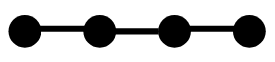
\includegraphics[width=4cm]{Line.png}
    \caption{\label{f1} $4$ node Line network.} 
    \end{figure}

    \begin{figure}
    \centering
    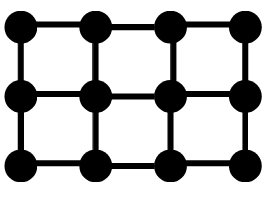
\includegraphics[width=4cm]{Grid.png}
    \caption{$12$ node Grid network. \label{f2}} 
    \end{figure}

    \begin{figure}
    \centering
    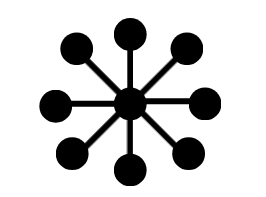
\includegraphics[width=4cm]{Star.png}
    \caption{$9$ node Star network. \label{f3}} 
    \end{figure}

    \begin{figure}
    \centering
    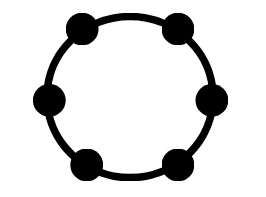
\includegraphics[width=4cm]{Circle.png}
    \caption{$6$ node Circle network. \label{f4}} 
    \end{figure}

    \section{Results}

    \subsection*{Fidelity}
    When we compare the networks against their receiver fidelity we obtain very similar results. Wherever due to the intrinsic nature of the simulator or future experimental results, we see no considerable speed up between classical forward transmission and the transmission of entanglement through a network. \ref{table_fidelity} 
    
    \begin{table}[!h] 
    \caption{Results obtained when comparing the fidelity of quantum vs classical network end-to-end message transmission in a line topology. These results are an average of 100 runs of the experiments.}
    \label{table_fidelity} 
    \centering 
    \begin{tabular}{|l || l|  l| l|} 
    \hline 
    Type of network & Number of nodes & Topology & Fidelity / 1 \\
    \hline 
    Classic & 3 & Line & 1.00\\ 
    Quantum & 3 & Line & 0.99\\ 
    Classic & 5 & Line & 0.99\\ 
    Quantum & 5 & Line & 0.99\\ 
    Classic & 10 & Line & 0.98\\ 
    Quantum & 10 & Line & 0.97\\ 
    Classic & 50 & Line & 0.96\\ 
    Quantum & 50 & Line & 0.94\\    
    Classic & 100 & Line & 0.94\\ 
    Quantum & 100 & Line & 0.94\\
    \hline 
    \end{tabular} 
    \end{table} 
    
    \subsection*{Speed}
    When we compare the networks against their timestamp distance we obtain very similar results. Wherever due to the intrinsic nature of the simulator or future experimental results, we see no considerable speed up between classical forward transmission and the transmission of entanglement through a network.\ref{table_speed} 
    
    \begin{table}[!h] 
    \caption{Results obtained when comparing the speed of quantum vs classical network end-to-end message transmission in a line topology. These results are an average of 100 runs of the experiments and they are described in NetSquid time units.}
    \label{table_speed} 
    \centering 
    \begin{tabular}{|l || l|  l| l|}  
    \hline 
    Type of network & Number of nodes & Topology & Speed (NetSquid timestamp units)  \\
    \hline 
    Classic & 3 & Line & 0.06\\ 
    Quantum & 3 & Line & 0.06 \\
    Quantum & 5 & Line & 2\\ 
    Quantum & 5 & Line & 2\\ 
    Classic & 10 & Line & 3\\ 
    Quantum & 10 & Line & 3\\ 
    Classic & 50 & Line & 4\\ 
    Quantum & 50 & Line & 4\\    
    Classic & 100 & Line & 6\\ 
    Quantum & 100 & Line & 6\\
    \hline 
    \end{tabular} 
    \end{table} 


    \section{Conclusion}
    
    \paragraph{In these results we observe very similar results for both the Quantum and Classical Networks. If we purely base of comparison of topology alone the results seem consistent across both types of networks. 
    We have three possible explanations for these results:
    - The lack of a specific tool designed to take into account the potential differences between these network's interactions with their mathematical topology.
    - A lack of correlation between the network's nature and it's performance against equivalent topologies.
    - A need to compare teleportation protocols for quantum networks against forwarding protocols in classical networks, given that these are the ideal simplest state of both networks.
    Further testing and analysis will be required to make a solid conclusion.
    Similarly further studies on the effects of various noise models within these topologies would be an interesting prolongation of this study. We would then expect a considerable speed up for quantum networks, and would be able to analyze wherever the disparity between results is affected by the topological setting.
    All relevant code is currently open source and available at \href{https://github.com/mgg39/Network-model-comparison}{Network model comparison}
    
    }

    \bibliographystyle{plain}
    \bibliography{References_bib.bib}

\end{document}